\documentclass[main.tex]{subfiles}
\begin{document}


\subsection{Nobili}

\paragraph{Tensor calculus}

The covariant derivative keeps account of the shifting of the basis vectors:

\begin{equation}
    \nabla_\mu A^\nu = \partial_\mu A^\nu + \Gamma^\nu _{\alpha \mu}  A^\alpha
\end{equation}

The rank-3 objects $\Gamma$ are called Christoffel symbols. They are not tensors! they depend on the choice of basis $e_\alpha$, and they satisfy $\nabla _\mu e_\alpha = \Gamma ^\nu _{\mu \alpha} e_\nu$. They are not intrinsic to the manifold.

If we have the metric (and make reasonable assumptions of the connection being torsion-free), they can be calculated as:

\begin{equation}
    \Gamma^\mu_{\nu \rho} = \frac{1}{2} g^{\mu \alpha} \qty(
    \partial_\rho g_{\alpha \nu} +
    \partial_\nu g_{\alpha \rho} -
    \partial_\alpha g_{\nu \rho}
    ) \label{eq:christoffel-symbols-from-metric}
\end{equation}

This also tells us that they are symmetric in the lower two indices: $\Gamma ^\mu _{\nu \rho} = \Gamma ^\mu _{\rho \nu}$.

The divergence of a vector field $A^\mu$ can be calculated as:

\begin{equation}
    \nabla_\mu A^\mu = \frac{1}{\sqrt{-g}}\partial_\mu \qty(\sqrt{-g}A^\mu) \label{eq:covariant-divergence}
\end{equation}

where $g$ is the determinant of the metric.

We can also define the Dalambertian operator $\square = \nabla_\mu \nabla^\mu = \nabla_\mu \partial^\mu$, which can only act on scalars, and it does so like:

\begin{equation}
    \square A = \nabla_\mu (\partial^\mu A) =  \frac{1}{\sqrt{-g}}\partial_\mu \qty(\sqrt{-g}\partial^\mu A)
\end{equation}

If we differentiate and antisymmetryze (so, take the rotor of) an antisymmetric tensor $F_{[\mu \nu]}$, the Christoffel symbols cancel:

\begin{equation}
    \nabla_{[\mu} F_{\nu\rho]} = \partial_{[\mu} F_{\nu\rho]}
\end{equation}

The derivative with respect to proper time is $\dv{}{\tau} = u^\mu \partial_\mu$.

\index{covariant acceleration}Covariant acceleration is defined as:

\begin{equation} \label{eq:covariant-acceleration-def}
    a^\nu = u^\mu \nabla_\mu u^\nu
\end{equation}

\paragraph{Curvature}

The curvature of spacetime is fully described by the Riemann curvature tensor, which is a fourth rank tensor: for any generic vector \(V^\mu\),

\begin{equation} \label{eq:riemann-tensor-def}
    R ^{\mu} _{\nu \rho \sigma} V^\nu \defeq [\nabla_\rho, \nabla_\sigma]   V^\mu
\end{equation}

It can be calculated using the Christoffel symbols, and while they are not tensors \(R ^{\mu} _{\nu \rho \sigma}\) is one. This result follows by direct computation from formula \eqref{eq:riemann-tensor-def}.

\begin{equation}
    R ^{\mu} _{\nu \rho \sigma} =
     \partial_\rho \Gamma^\mu_{\nu \sigma}
    -\partial_\sigma \Gamma^\mu_{\nu \rho}
    +\Gamma^\mu_{\rho \lambda} \Gamma ^{\lambda} _{\sigma \nu}
    -\Gamma^\mu_{\sigma \lambda} \Gamma ^{\lambda} _{\rho \nu}
\end{equation}

The Christoffel symbols can be nonzero if we choose certain coordinates even for flat spacetime, but the Riemann tensor is zero iff the spacetime is flat.

The Riemann tensor satisfies the following identities \cite[eqs. 8.45 and 8.76]{MisnerThorneWheeler:1973}:

\begin{subequations}
\begin{align}
  \nabla _{[\lambda} R_{\mu\nu]\rho \sigma} &= 0 \label{eq:bianchi-identities}  \\
  R_{\mu\nu\rho\sigma} &= R_{[\mu\nu][\rho\sigma]} = R_{[\rho\sigma][\mu\nu]}  \\
  R_{[\mu\nu\rho\sigma]} &= 0 = R_{\mu[\nu\rho\sigma]}
\end{align}
\end{subequations}

If we define the Ricci tensor \(R_{\mu\nu} = R^\rho_{\mu \rho \nu}\) and the curvature scalar \(R = R_{\mu\nu}g^{\mu\nu}\), we can rewrite \eqref{eq:bianchi-identities}  as \(\nabla_\mu R = 2 \nabla_\nu R^{\nu}_{\mu}\).

\paragraph{Geodesics}

If we have a path $x^\mu(\lambda)$, we would like to see if it is a geodesic, that is, if it is stationary with respect to path length. To do this we can stationarize the action corresponding to the lagrangian $\Lagr (x, \Dot{x}) = g_{\mu\nu} \Dot{x}^\mu \Dot{x}^\nu$ (where we use $\Dot{x} = \dv*{x}{\lambda}$). The Lagrange equations then are:

\begin{equation}
    \Ddot{x}^\mu + \Gamma^\mu_{\nu\rho} \Dot{x}^\nu \Dot{x}^\rho = 0
\end{equation}

Where $\Gamma$ are the Christoffel symbols, which can be calculated by differentiating the metric, as shown in \eqref{eq:christoffel-symbols-from-metric}. $\Lagr$ is an integral of these Lagrange equations.

If the parameter $\lambda$ is taken to be the proper time $s$, then the equation is

\begin{equation}
    \dv{u^\mu}{s} + \Gamma^\mu _{\nu\rho} u^\nu u^\rho = 0
\end{equation}

Notice that this is equivalent to the covariant acceleration \eqref{eq:covariant-acceleration-def} being zero.

\paragraph{Fermi-Walker transport}

Take a general vector field \(V ^{\mu} (s)\) defined along a curve, with its tangent vector \(u^\mu\) whose covariant acceleration is \(a^\mu\).
Then we say that \(V^\mu\) is transported according to Fermi-Walker iff it satisfies

\begin{equation}
    \dot{V}^\mu  = u^\nu \nabla_\nu V^\mu
    = 2 V_\rho u^{[\mu} a^{\rho]}
\end{equation}

This condition is always satisfied by \(V^\mu = u^\mu\), since \(a^\mu u_\mu = 0\), whether or not the curve is a geodesic. The tangent vector is \emph{parallel} transported only for geodesics.

The justification of this definition is the fact that we want the transformations of our our tetrad to be infinitesimal Lorentz boosts, which are generated by antisymmetric tensors, and we want to prohibit any rotations in the plane orthogonal to \(a^\mu\) and \(u^\mu\)

\paragraph{Tetrads and projectors} \label{par:tetrads}

We want to work in a reference in which the velocity $u^\mu$ is purely timelike. This can always be found by the equivalence principle. Such a reference can be completed into what  is called a tetrad, for which the metric becomes the Minkowski metric in a neighbourhood of the point we consider.

We call the velocity \(u^\mu = V^\mu _{(0)}\), and add to it three other vectors \(V^\mu_{(i)}\) such that

\begin{equation}
    g_{\mu\nu} V^\mu _{(\alpha)} V^\nu _{(\beta)} = \eta_{(\alpha) (\beta)}
\end{equation}

where the brackets around the indices denote the fact that they label four vectors, not the components of a tensor.

We can choose the vectors \(V_{(i)}^\mu\) so that they are Fermi-Walker transported along the worldline defined by \(u^\mu\): this allows us to find the relativistic equivalent of a nonrotating frame of reference.

It is useful to project tensors onto the space-like and time-like subspaces defined by our tetrad (and we wish to do so in a coordinate-independent manner,  so just taking the 0th and $i $-th components in the tetrad will not suffice). We therefore define the projectors:

\begin{equation}
    h_{\mu \nu} = u_\mu u_\nu + g_{\mu \nu} \qquad \pi_{\mu\nu} = -u_\mu u_\nu
\end{equation}

respectively onto the space- and time-like subspaces.

\paragraph{Killing vector fields}

Following \cite[section 25.2, page 650]{MisnerThorneWheeler:1973}.
Say there is a certain direction (for simplicity, along one of our coordinate axes) along which the metric is preserved: an \(\widetilde{\alpha}\) such that \(\partial_{\widetilde{\alpha} g_{\mu\nu}}\).

Then the metric properties of curves along the manifold are unchanged if we shift their coordinate representation by a constant along the \(\widetilde{\alpha}\) coordinate axis.

Let us call the direction of this translation \(\xi^\mu = \delta^\mu_{\widetilde{\alpha}}\) if we use this coordinate system. It can be shown by direct computation that

\begin{equation} \label{eq:killing-vector-identity}
    \nabla_{\nu} \xi_\mu = \frac{1}{2} \qty(\partial_{\widetilde{\alpha}}
    g_{\mu\nu} + \partial_\nu g_{\mu\widetilde{\alpha}} -
    \partial_\mu g_{\nu \widetilde{\alpha}})
\end{equation}

but by hypothesis the first term on the RHS of \eqref{eq:killing-vector-identity} is zero, therefore we have shown that \(\nabla_{\nu} \xi_\mu = \nabla_{[\nu} \xi_{\mu]}\) in this coordinate frame, but since this is a covariant equation it extends to every other one.

It can also be seen this way that \(\nabla_{(\nu} \xi_{\mu)}=0\): this is called \emph{Killing's equation}. This is useful since: given a geodesic \(x^\mu(\lambda)\), for which we define \(u^\mu = \dv*{x^\mu}{\lambda} \), it must be the case that \(u^\nu \nabla_\nu u^\mu = 0 \). Then, the component of \(u^\mu\) along \(\xi^\mu\) (\(u^{\widetilde{\alpha}} = u^\mu \xi_\mu\)) is conserved:

\begin{equation}
    \dv{}{\lambda} \qty(u^\mu \xi_\mu) = u^\nu \nabla_\nu \qty(u^\mu \xi_\mu)
    = \cancelto{0}{\xi^\mu u^\nu \nabla_\nu u_\mu} + \cancelto{0}{u^\nu u^\mu \nabla_\nu \xi_\mu} \equiv 0
\end{equation}

\paragraph{Lie derivative}

Following \cite[section 6]{Taub:1978}. The Lie derivative of a generic tensor \(T^{\mu_1 \dots \mu_n} _{\nu_1 \dots \nu_m}\) along a vector \(\xi^\mu\) is defined as:

\begin{equation}
    \Lie_{\xi} T^{\mu_1 \dots \mu_n} _{\nu_1 \dots \nu_m} \defeq
    \xi^\rho \nabla_\rho T^{\mu_1 \dots \mu_n} _{\nu_1 \dots \nu_m}
    + \sum_{i=1}^{m} T^{\mu_1 \dots \mu_n} _{\nu_1 \dots \nu_{i-1} \rho \nu_{i+1} \dots \nu_m} \nabla_{\nu_i} \xi^\rho
    - \sum_{i=1}^{n} T^{\mu_1 \dots \nu_{i-1} \rho \nu_{i+1} \dots \mu_n} _{\nu_1 \dots  \nu_m} \nabla_{\rho} \xi^{\mu_i}
\end{equation}

Some special cases are: a scalar \(\Lie _\xi f = \xi^\rho \partial_\rho f \), a vector \(\Lie _\xi u^\mu = \xi^\rho \nabla_\rho u^\mu -u^\rho \nabla_\rho \xi^\mu\), and  an antisymmetric covariant two-tensor \(\omega_{\mu\nu} = \omega_{[\mu \nu]}\) which represents a closed form \(\nabla_{[\mu} \omega_{\nu \rho]} = 0\) we have \(\Lie _\xi \omega_{\mu\nu} =2\nabla_{[\nu} \qty( \omega_{\mu] \rho} \xi^\rho )\)

\paragraph{Useful metrics}

The simplest physically relevant one is the Schwarzschild metric. It describes a spherically symmetric object of mass $M$, in spherical coordinates. Defining $\Phi = -M/r$, we have:

\begin{equation}
    \dd{s}^2 = -(1+2\Phi)\dd{t}^2 + \frac{1}{1+2\Phi} \dd{r}^2
    + r^2 \qty(\dd{\theta}^2 + \sin^2\theta \dd{\varphi}) \label{eq:schwartzshild-line-element}
\end{equation}

or, equivalently,

\begin{equation}
    g_{\mu\nu} =  \diag\qty(-(1+2\Phi),\, \frac{1}{1+2\Phi},\, r^2,\, r^2 \sin ^2 \theta )
\end{equation}

We can see that it approaches the flat metric $\eta_{\mu\nu} = \diag\qty(-, +, +, +)$ in the limit $M\rightarrow 0$. Its determinant is $g = -r^4 \sin^2 \theta$.

\paragraph{Fluid mechanics}

In usual relativistic single-body mechanics, we use the 4-velocity $u^\mu$ and the corresponding 4-momentum $p^\mu = m u^\mu$. The 0-th component of this vector is the energy of the body, while the $i$-th components are its momentum: we then have $p^\mu p_\mu = m^2 = E^2 - \abs{p}^2$.

When dealing with a continuum, we will have a certain density of particles per unit of volume, we call this $n$. The current of particles is then $N^\mu = n u^\mu$. If these particles have a certain rest mass $m_0$, we can then define the vector $\rho_0 u^\mu = m_0 n u^\mu = m_0 N^\mu$.

This satisfies a conservation equation: $\nabla_\mu(\rho_0 u^\mu) = 0$.

Particles in a fluid can have three kinds of energy we concern ourselves with: mass, kinetic energy and other forms of energy (thermal, chemical, nuclear\dots).
We can always perform a change of coordinates to bring us to a frame in which the kinetic energy is zero. We write the sum of the other two forms of energy as $\rho = \rho_0 (1+\epsilon)$. So, $\epsilon$ is the ratio of the internal non-mass energy to the mass.

Now, the vector $\rho u^\mu$ describes the flux of energy.
We can then write the equation for the conservation of momentum:

\begin{equation}
    f^\mu = \nabla_\nu (\rho u^\mu u^\nu)
\end{equation}

\paragraph{Ideal fluids}

They are fluids with \(\eta=\xi=\kappa=0\), that is, without viscosity (neither compressive nor shear) nor heat transmission.
They are described by the following stress-energy tensor:

\begin{equation}
    T^{\mu\nu} = \rho u^\mu u^\nu + p h^{\mu\nu}
\end{equation}

\paragraph{Spherical accretion}

We work with the Schwarzschild metric \eqref{eq:schwartzshild-line-element}; we treat a fluid with 4-velocity $u^\mu$ in spherical coordinates, since the problem we are looking at is stationary and spherically symmetric the velocity is:

\begin{equation}
    u^\mu = \begin{pmatrix}
        \gamma^2 / y\\
        yv\\
        0\\
        0
    \end{pmatrix}
\end{equation}

where we define the Lorentz factor as usual, $\gamma = \qty(1-v^2)^{-1/2}$, and $y=\gamma \sqrt{1+2\Phi}$ is the ``energy-at-infinity per unit rest mass'' (see \cite[equation 3]{ThorneFLammmangZytkow:1981feb}).

The conservation of mass holds: if $\rho_0$ is the rest mass density of the fluid, we must have $\nabla_\mu \qty(\rho_0 u^\mu) =0$. This, using the formula for covariant divergence \eqref{eq:covariant-divergence}, yields:

\begin{equation} \label{eq:integral-continuity}
    \dv{}{r} \qty(\rho_0 yvr^2) = 0
\end{equation}

\(\dv*{Q}{r} = 0\) is equivalent to \(\dv*{\log Q }{\log r} = 0 \), therefore we can recast \eqref{eq:integral-continuity} into

\begin{equation} \label{eq:differential-continuity}
  \dv{\log \rho_0}{\log r} +
  \dv{\log yv}{\log r} + 2 = 0
\end{equation}

In the newtonian limit both $\gamma$ and $y$ approach 1; also, the infalling mass rate $\Dot{M}$ at a certain radius is $\rho_0 (r) v(r) 4\pi r^2$. Then, by continuity to the newtonian limit, the quantity which is constant wrt the radius must be $\Dot{M} / (4\pi)$: therefore

\begin{equation}
  \dot{M} = 4 \pi\rho_0 yvr^2
\end{equation}

We also have the Euler equation:

\begin{equation} \label{eq:relativistic-euler}
    (p+\rho) a^\mu = - h^{\mu \nu} \partial_\nu p
\end{equation}

The only interesting component of this is the radial one, so we need to calculate \(a^1 = u^\mu \nabla_\mu u^1 = \dv*{u^1}{\tau} + \Gamma^1_{\mu \nu} u^\mu u^\nu \). To do this we will need the radial Schwarzschild Christoffel coefficients:

\begin{equation}
  \Gamma^1_{\mu \nu} = \left[\begin{matrix}\frac{M \left(- 2 M + r\right)}{r^{3}} & 0 & 0 & 0\\0 & \frac{M}{r \left(2 M - r\right)} & 0 & 0\\0 & 0 & 2 M - r & 0\\0 & 0 & 0 & \left(2 M - r\right) \sin^{2}{\left(\theta \right)}\end{matrix}\right]
\end{equation}

while the proper-time derivative is \(\dv*{}{\tau} = u^\mu \partial_\mu = yv\partial_1\).
Plugging in the expression for the only relevant component of \(h^{\mu\nu}\), \(h^{11} = g^{11} + u^1 u^1 = (1 + 2 \Phi) (1 + v^2 \gamma^2) = y^2\)
we get, after lengthy computation,

\begin{equation}
  a^1 = y^2 \qty(\gamma^2 v \dv{v}{r} + \frac{M}{(1+ 2 \Phi) r^2})
\end{equation}

Substituting this into the (radial component of the) Euler equation \eqref{eq:relativistic-euler} we get

\begin{subequations}
\begin{align}
  (p + \rho) y^2 \qty(\gamma^2 v \dv{v}{r} + \frac{M}{(1+ 2 \Phi) r^2}) &= - h^{1 1} \partial_1 p = - y^2 \partial_1 p \\
   \gamma^2 v \dv{v}{r} + \frac{M}{(1+ 2 \Phi) r^2} + \frac{1}{p + \rho} \dv{p}{r} &= 0
  \label{eq:ideal-euler}
\end{align}
\end{subequations}

\begin{greenbox}
  In equations 3.12.7, 8 in \cite{Nobili:2000} there is most definitely a sign error.
\end{greenbox}

We also have the equation for the variation of the total internal energy, which holds for ideal fluids at constant entropy:

\begin{equation} \label{eq:enthalpy-definition}
    \dv{\rho}{\tau} = \frac{p+\rho}{\rho_0} \dv{\rho_0}{\tau}
    \qquad
    \text{or}
    \qquad
    \pdv{\rho}{\rho_0} = \frac{p + \rho}{\rho_0} \defeq h
\end{equation}

(where we have defined $h$, the specific enthalpy).
From these we can show that

\begin{claim}
The quantity $\gamma h \sqrt{1+2\Phi} = yh$ , is a constant of motion.
\end{claim}

\begin{proof}
First of all, by direct computation it can be shown that

\begin{equation} \label{eq:log-y-conservation}
  \gamma^2 v \dv{v}{r} + \frac{M}{(1+ 2 \Phi) r^2} = \dv{\log y }{r}
\end{equation}

Then, following \textcite[section 6.3]{Gourgoulhon:2006bn} we find that \(\dd{p} = \rho_0 \dd{h}\) in the isentropic case, therefore

\begin{equation} \label{eq:log-h-conservation}
  \frac{1}{\rho + p} \dv{p}{r}  =  \dv{\log h}{r}
\end{equation}

we can substitute the results in \eqref{eq:log-y-conservation} and \eqref{eq:log-h-conservation} into \eqref{eq:ideal-euler}:

\begin{equation}
  \dv{\log h}{r} + \dv{\log y }{r} = \dv{\log (hy) }{r} = 0
\end{equation}

\end{proof}

In the nonrelativistic, weak-field limit this  becomes the classical conservation of density of energy:

\begin{equation}
    \gamma h \sqrt{1+2\Phi} \approx \frac{p}{\rho_0} + \frac{v^2}{2} - \frac{M}{r} + \epsilon = \const
\end{equation}

Also, we can rewrite the last term of the Euler equation \eqref{eq:ideal-euler} using \eqref{eq:enthalpy-definition}  as:

\begin{equation}
  \frac{\partial_1 p}{p + \rho} =
  \frac{\rho_0}{\rho_0} \frac{\partial_1 p}{p + \rho} =
  \frac{1}{\rho_0} \pdv{p}{\rho} \pdv{\rho_0}{\rho}
  \pdv{\rho}{p}   \partial_1 p =
  \frac{v_s^2}{\rho_0} \partial_1\rho_0
\end{equation}

where we define the speed of sound \(v_s^2 = (\pdv*{p}{\rho})_s\) (the index \(s\) means the derivative is to be taken at constant entropy, and for an adiabatic process).

This can be rewritten as

\begin{equation}
  \dd{p} = \pdv{p}{\rho} \pdv{\rho}{\rho_0} \dd{\rho_0} = v_s^2 h \dd{\rho_0}
\end{equation}

\begin{greenbox}
  Somehow in \cite[page 175]{Nobili:2000} this becomes:

  \begin{equation}
    \dv{\log p }{\log r} = \rho_0 v_s^2 \dv{\log \rho_0}{\log r }
  \end{equation}

  but it seems to me it should be

  \begin{equation}
  \dv{\log p }{\log r} = \frac{p+\rho}{p} v_s^2 \dv{\log \rho_0}{\log r }
  \end{equation}
\end{greenbox}

Coming back to \eqref{eq:relativistic-euler},  we get:

\begin{equation}
  \gamma^2 v \dv{v}{r} + \frac{M}{(1+ 2 \Phi) r^2}
  + \frac{v_s^2 }{\rho_0}\dv{\rho_0}{r} = 0
\end{equation}

We can replace every occcurence of \((\partial x) / x \) with \(\partial \log x \):

\begin{subequations}
\begin{align}
  \gamma^2 v^2 \dv{\log v}{r} + \frac{M}{(1+ 2 \Phi) r^2} + v_s^2 \dv{\log \rho_0}{r}  &= 0 \\
  \frac{\gamma^2 - 1}{r}  \dv{\log v}{\log r} + \frac{M}{(y^2/\gamma^2) r^2}
  + \frac{v_s^2}{r} \dv{\log \rho_0}{\log r}  &= 0  \\
  % \frac{1 - (1-v^2)}{1}  \dv{\log v}{\log r} + \frac{M}{(y^2) r}
  % + (1-v^2)\frac{v_s^2}{1} \dv{\log \rho_0}{\log r}  &= 0 \\
  v^2  \dv{\log v}{\log r} + \frac{M}{y^2 r}
  + (1-v^2) v_s^2 \dv{\log \rho_0}{\log r}  &= 0
\end{align}
\end{subequations}

\begin{greenbox}
  Are the eqrefs at page 174 in \cite{Nobili:2000} wrong? Equations 2.7.3, 5 seem not to be related at all...

  Somehow this equation comes up:

  \begin{equation}
    \dv{\log \rho_0 }{r} + \gamma^2 v^2 \dv{\log v }{r}  + \frac{2 v^2}{r} + \frac{M}{(1+2 \Phi) r^2} = 0
  \end{equation}

  and we wind up with the system

  \begin{subequations}
  \begin{align}
    (v^2-v_s^2) \dv{\log \rho_0}{\log r} &= - 2v^2 + \frac{M}{y^2 r}  \\
    (v^2-v_s^2) \dv{\log yv }{\log r} &=  2v_s^2 - \frac{M}{y^2 r}  \\
    \dv{\log p }{\log r} &= \rho_0 v_s^2 \dv{\log \rho_0}{\log r }
  \end{align}
  \end{subequations}

  but I do not see at all how to get to it, it does not seem to work!
  If we add the first two equations we get back \eqref{eq:differential-continuity}...
\end{greenbox}

\begin{greenbox}
  Typo in \cite[page 175]{Nobili:2000}: shouldn't it be ``il movimento avviene nella direzione opposta (\(v>0, \dot{M}>0)\))''?
\end{greenbox}

\subsection{Taub}

This section summarizes my study of A. H. Taub's review of relativistic fluid dynamics, \cite{Taub:1978}.

\paragraph{Nonrelativistic}

Nonrelativistic fluid mechanics are described by the equations:

\begin{subequations}
\begin{align}
    \partial_t \rho + \partial_i (\rho v^i) &= 0 &\text{conservation of mass} \\
    \rho \qty(\partial_t v^i + v^j \partial_j v^i) &= \partial_j T^{ij} &\text{conservation of momentum}  \\
    \rho \partial_t E + v^i \partial_i E &= \partial_i \qty(T^{ij}v_j + \kappa\partial^i T) &\text{conservation of energy}
\end{align}
\end{subequations}

where $\rho$ is the density of the fluid,
$v^i$ are the components of its velocity,
$T^{ij}$ is the stress tensor (or, equivalently, the space-like components of the energy-momentum tensor),
$E$ is the energy of the fluid,
$\kappa$ is the thermal conductivity,
$T$ is the temperature of the fluid.

The nonrelativistic stress tensor can be written as:

\begin{equation}
    T_{ij} = -(p + \xi \partial_k v^k ) \delta_{ij} + \eta \partial_{(i} v_{j)}
\end{equation}

where $p$ is the (isotropic) pressure, $\eta$ the viscosity, $\xi$ is the compression viscosity. We are assuming that the normal stresses are only those exerted by pressure, so the diagonal terms $T_{ii}$ (not summed) must just be $-p$. So, the term $-\xi \partial_k v^k$ must equal $\eta \partial_{(i} v_{i)} = 2\eta \partial_i v_i$ (not summed). Therefore, by isotropy, $\xi = 2\eta/3$.

Note that we are working in Euclidean 3D space, so the metric is the identity and upper and lower indices are equivalent.

The energy is a sum of kinetic and specific energy:

\begin{equation}
    E = v^i v_i /2 + \varepsilon
\end{equation}

where $\varepsilon$ is the specific energy (of a type that is different from kinetic) per unit mass.

\paragraph{Surfaces in space-time and acceleration decomposition}

Following \cite[section 4]{Taub:1978}
We look at 4D space time in 3D space-like slices: if we have a fluid moving with velocity \(u^\mu\), we can look at the solutions of the associated differential equation: \(x^\mu (\xi^i, s)\), where \(\xi^i\) are the 3D coordinates of the starting position and \(s\) is the time at which we look at the solution. Then we can look at the ``starting'' hypersurface \(\Sigma = \qty{x^\mu (\xi^i, 0)}\).

Say we have a curve \(\xi^i(\tau)\) in \(\Sigma\). Then we can look at the two-dimensional surface defined by the evolution of \(\xi^i(\tau)\): \(x^{\mu} (\xi^i(\tau), s) = x^\mu (\tau, s)\). If we define the ``spatial'' tangent vector \(\lambda^\mu = \dv*{x^\mu}{\tau} \), it follows from Schwarz's theorem that:

\begin{equation} \label{eq:schwarz-spacetime-tube}
    \pdv{x^\mu}{\tau}{s} =
    \pdv{x^\mu}{s}{\tau}
    \implies
    \pdv{u^\mu}{\tau} = \pdv{\lambda^\mu}{s}
\end{equation}

Now let us take the spatial vectors of an orthonormal Fermi-Walker transported tetrad \(V^\mu_{(a)}\) as described in \Nameref{par:tetrads}, and express \(\lambda^\mu\) in this frame: its covariant components will be

\begin{equation} \label{eq:tetrad-components-lambda}
    X_{(a)} = V_{(a)\mu} \lambda^\mu
\end{equation}

If we differentiate \eqref{eq:tetrad-components-lambda} wrt \(s\), and use \eqref{eq:schwarz-spacetime-tube} with the fact that \(\dv{}{\tau} = \lambda^\mu \nabla_\mu \), we get:

\begin{subequations}
\begin{align}
    \dv{X_{(a)}}{s} &= \dv{V_{(a)\mu}}{s} \lambda^\mu + V_{(a)\mu} \dv{\lambda^\mu}{s}  \\
    &= V_{(a)}^\rho \cancelto{0}{\lambda^\mu u_\mu} a_\rho - \cancelto{0}{V_{(a)}^\rho  u_\rho} \lambda^\mu a_\mu
    + V_{(a)}^\nu \nabla_\mu u_\nu  \\
    &= V^\rho _{(a)} \lambda^\mu \nabla_\mu u_\rho  \\
    &= \qty(\nabla_\mu u_\rho) V^\rho_{(a)} V^{\mu}_{(b)} X^{(b)}
\end{align}
\end{subequations}

where in the last step we expressed everything wrt the tetrad coordinate system. Therefore, in those cordinates, the evolution of the components \(X^{(a)}\) is linear, and defined by the tetrad components of the two-form \(\nabla_\mu u_\nu\). So, we want to decompose this tensor:

\begin{equation} \label{eq:covariant-acceleration-decomposition}
    \nabla_\sigma u_\tau =
    \underbrace{\omega_{\sigma \tau}}_{\substack{\text{spatial} \\ \text{rotation}}}
    + \underbrace{\sigma_{\sigma\tau}}_{\substack{\text{spatial} \\ \text{shear}}}
    + \underbrace{\frac{1}{3} \theta h_{\sigma\tau}}_{\substack{\text{spatial} \\
    \text{compression}}}
    - \underbrace{ a_\tau u_\sigma}_{\substack{\text{temporal} \\ \text{acceleration}}} \\
\end{equation}

\begin{enumerate}
    \item \(\theta = \nabla_\mu u^\mu\) is the bare trace of the tensor, corresponding to the expansion velocity;
    \item \(a_\mu = u^\nu \nabla_\nu u^\mu\) is the covariant acceleration;
    \item \(\sigma_{\sigma \tau} = \qty(\nabla_{(\mu} u_{\nu)}) h^\mu_\sigma h^\nu _\tau - \frac[i]{1}{3} \theta h_{\sigma \tau} = \nabla_{(\sigma} u_{\tau)} + a_{(\sigma} u_{\tau)} - \frac[i]{1}{3} \theta h_{\sigma \tau} \) is the spatial symmetric trace-free part of the tensor, that is, the shear stress;
    \item \(\omega_{\sigma \tau} = h^\nu_\sigma h^\mu_\tau \nabla_{[\nu} u_{\mu]} = \partial_{[\tau} u_{\sigma]} + a_{[\tau} u_{\sigma]}\) is the spatial rotation tensor.
\end{enumerate}

We can describe the rotation with a ``vorticity vector'':

\begin{equation}
    \omega^\mu = \frac{1}{2 \sqrt{-g}} \varepsilon^{\mu\nu\sigma\tau} u_\nu \partial_\tau u_{\sigma} = \frac{1}{2} \eta^{\mu\nu\sigma\tau} u_\nu \partial_\tau u_{\sigma}
\end{equation}

where we define the fully antisymmetric, covariant tensor \(\eta^{\mu\nu\sigma\tau} = \varepsilon^{\mu\nu\sigma\tau} / \sqrt{-g} \). With its indices lowered, it is
\(\eta_{\mu\nu\sigma\tau} = - \varepsilon_{\mu\nu\sigma\tau} \sqrt{-g} \).

Note, from \cite[pages 51--52]{Carroll:1997ar}: this is the volume form of the manifold, and it is defined this way since \(g\) is a \emph{tensor density} of weight $-2$, while the bare Levi-Civita symbol is a density of weight $+1$.

\begin{greenbox}
  The signs in \cite[]{Taub:1978} and \cite[]{Carroll:1997ar} seem to disagree though!
\end{greenbox}

By the antisymmetry in the definition we can immediately see that \(\omega^\mu u_\mu=0\). It holds that \(\omega^\mu \equiv 0 \iff u_\mu = \rho \partial_\mu f \) (locally!) for scalar \(\rho\), \(f\), since this is equivalent to \(u_\mu\) being a closed form.

\(\omega_\mu\) and \(\omega_{\mu \nu}\) are ``dual'' in the sense that

\begin{equation}
    \omega _{\sigma\tau} = u^\mu \omega^\nu \eta_{\mu \nu \sigma \tau}
\end{equation}

and some other useful identities can be found in equations 7.5 through 7.7 of \cite[]{Taub:1978}.

\paragraph{Wave velocity}

Following \cite[section 5]{Taub:1978}.

An equation in the form \(\varphi (x^\mu) = 0\) defines a 3D surface \(\Sigma\); its constant-\(x^0\) slices are 2D surfaces. We can decompose \(\partial_\mu \varphi\) in a component proportional to the velocity, \(a u_\mu\), and one which is orthogonal to it, \(W_\mu = h^\sigma_\mu \partial_\sigma \varphi\). Then \(W_\mu W^\mu = h^\sigma_\mu  h_\beta^\mu \partial_\sigma \varphi \partial^\beta \varphi = h^{\sigma\beta} \partial_\sigma \varphi \partial_\beta \varphi\)
by the idempotency of the projector \(h\).
Thus we can see that \(W^2 \geq 0\), therefore it is a spacelike vector. We can define its corresponding unit vector: \(W^\mu = t^\mu \sqrt{W^\nu W_\nu}\).

We can choose a velocity \(v\) such that \(k^\mu = u^\mu - v t^\mu\) is parallel to \(\Sigma\), or \(k^\mu \partial_\mu \varphi = 0\). If this condition is satisfied, then \(v\) is the wave velocity of \(\Sigma\) as measured by an observer with velocity \(u^\mu\).

\begin{figure}[ht]
  \centering
  \incfig{figures/taub_wave_velocity}
  \caption{Wave velocity diagram}
  \label{fig:taub_wave_velocity}
\end{figure}

Now, we can multiply the equation \(k^\mu = u^\mu - v t^\mu\) by \(\partial_\mu \varphi\): we get \(v t^\mu \partial_\mu \varphi = u^\mu \partial_\mu \varphi\). What multiplies \(v\) in the LHS of this equation is the length of the spatial component of \(\partial_\mu \varphi\), or \(\sqrt{h^{\mu\nu} \partial_\mu \varphi \partial_\nu \varphi}\).
Using the definition of \(h ^{\mu \nu} \), we can arrive at

\begin{equation} \label{eq:lorentz-factor-wave-velocity}
    \gamma^{-2} = 1 - v^2 = \frac{g^{\mu\nu} \partial_\mu \varphi \partial_\nu \varphi}{h^{\mu\nu} \partial_\mu \varphi \partial_\nu \varphi}
\end{equation}

The denominator in \eqref{eq:lorentz-factor-wave-velocity} is positive, so we can see that \(1-v^2\) is positive iff \(\partial_\mu \varphi\) is spacelike, and \(v^2 = 1\) iff it is null.

If we are dealing with a timelike surface \(\Sigma\), or equivalently \(\partial_\mu \varphi\) is spacelike, then we define \(n^\mu \propto \partial_\mu \varphi\) such that \(n^\mu n_\mu = 1\) and we find:

\begin{equation}
    v = \frac{u^\mu \partial_\mu \varphi}{\sqrt{h^{\mu\nu} \partial_\mu \varphi \partial_\nu \varphi}}
    = \frac{u^\mu n_\mu}{\sqrt{h^{\mu\nu} n_\nu n_\mu}}
    = \frac{u^\mu n_\mu}{\sqrt{1 + (u^\mu n_\mu)^2}}
\end{equation}

From this it can be shown that \(1-v^2 = (1+(u^\mu n_\mu)^2)^{-1}\), and then \(v \gamma = u^\mu n_\mu\).

\paragraph{Relativistic non-ideal fluid dynamics}

The dynamics of the fluid are described by the conservation of the stress-energy tensor \(\nabla_\mu T ^{\mu \nu} =0\) and the conservation of mass \(\nabla_\mu (\rho u^\mu) =0\).

Any stress-energy tensor can be decomposed in its space and time-like parts in the local rest frame of the fluid:

\begin{equation} \label{eq:stress-energy-tensor-decomposition}
    T_{\mu \nu} = w u_\mu u_\nu + w_\mu u_\nu + u_\mu w_\nu + w _{\mu \nu}
\end{equation}

where

\begin{subequations} \label{eq:components-stress-energy-tensor}
\begin{align}
  w &=  T _{\mu \nu} u^\mu u^\nu = \rho_0 (1 + \varepsilon) \\
  w_\mu &= T _{\nu \sigma} h^\sigma _\mu u^\nu  = -\kappa h_\mu ^\sigma  \qty(\partial_\sigma T + T a_\sigma)\\
  w_{\mu \nu} &= T_{\rho \sigma} h^\rho _\mu h^\sigma_\nu = \qty(p - \xi \theta) h_{\mu \nu} - 2 \eta \sigma_{\mu \nu}
\end{align}
\end{subequations}

For the definition of the acceleration, vorticity etc. see equation \eqref{eq:covariant-acceleration-decomposition}.
As in the nonrelativistic section \(\eta\) is the viscosity, \(\xi\) is the compression viscosity,  \(\kappa\) is the thermal conductivity, \(T\) is the temperature field, \(p\) is the pressure, \(\rho_0\) is the rest mass density while \(\rho = \rho_0 (1 + \varepsilon)\) is the rest energy.

It holds \cite[]{Taub:1948} that:

\begin{equation}
    0
    \leq 3p
    \leq \frac{3}{2}p + \sqrt{\qty(\frac{3}{2}p)^2 + \rho_0^2}
    \leq \rho = \rho_0 (1 + \varepsilon)
    \leq \rho_0 + 3p
\end{equation}

Because of the conservation of the stress-energy tensor, we have:

\begin{equation} \label{eq:velocity-stress-energy-tensor-identity}
    \nabla_\nu \qty(u_\mu T ^{\mu \nu}) = T^{\mu \nu} \nabla_\nu u_\mu
\end{equation}

Let us also consider the expression of the differential entropy:

\begin{equation} \label{eq:differential-entropy}
    T\dd{S} = \dd{\varepsilon} + p \dd{\frac{1}{\rho_0}}
\end{equation}

\begin{claim}
    We can mold equation \eqref{eq:velocity-stress-energy-tensor-identity} into a version of the second principle of thermodynamics

    \begin{equation} \label{eq:second-principle-thermodynamics}
        T \nabla_\mu S^\mu = \xi \theta^2 + 2 \eta \sigma_{\mu\nu} \sigma^{\mu\nu} + \frac{w^\mu w_\mu}{\kappa T} \geq 0
    \end{equation}

    where we define \(S^\mu = \rho_0 S u^\mu + w^\mu /T\).
\end{claim}

\begin{proof}
    We will need the decompositions of
    the derivative of velocity \eqref{eq:covariant-acceleration-decomposition},
    of the stress-energy tensor \eqref{eq:stress-energy-tensor-decomposition}, \eqref{eq:components-stress-energy-tensor},
    the expression of differential entropy \eqref{eq:differential-entropy}
    and the conservation of mass \(\nabla_\mu (\rho_0 u^\mu) = 0\).

    First of all, the LHS of \eqref{eq:velocity-stress-energy-tensor-identity} can be greatly simplified by noticing that \(u^\mu w_\mu = u^\mu w_{\mu \nu} = 0\), so it becomes

    \begin{subequations}
    \begin{align}
        \nabla_\nu \qty(u_\mu T ^{\mu \nu}) &= \nabla_\nu \qty( w \underbrace{u_\mu u^\mu}_{-1} u^\nu + \underbrace{u_\mu w^\mu}_{0} u^\nu + \underbrace{ u_\mu u^\mu}_{-1} w^\nu + \underbrace{u_\mu w ^{\mu \nu}}_{0}) \\
         &= \nabla_\nu \qty(- u^\nu \rho_0 (1 + \varepsilon) + \kappa h_\sigma^\nu \qty(\partial^\sigma T + T a^\sigma)) \\
         &=  - \rho_0 u^\nu \nabla_\nu \varepsilon + \kappa \nabla_\nu \qty( h_\sigma^\nu \qty(\partial^\sigma T + T a^\sigma))  \\
         &= - \rho_0 u^\nu \partial_\nu \varepsilon + \kappa \qty( \nabla_\nu \qty(\partial^\nu T + T a^\nu) + \nabla_\nu \qty(u^\nu u_\sigma \qty(\partial^\sigma T + T a^\sigma)))  \\
         &= - \rho_0 u^\nu \partial_\nu \varepsilon + \kappa \qty(
         \qty(\nabla^\nu + 2 a^\nu + \theta u^\nu + u^\alpha u^\nu \nabla_\alpha
         ) \partial_\nu T + T \nabla_\nu a^\nu
         )
    \end{align}
    \end{subequations}

    The RHS of \eqref{eq:velocity-stress-energy-tensor-identity} instead becomes:

    \begin{subequations}
    \begin{align}
      \qty(\nabla_\nu u_\mu) T^{\mu \nu} &=
      \qty(\omega_{\nu \mu} + \nu_{\nu\mu} + \frac{1}{3} \theta h_{\nu\mu}
      -  a_\mu u_\nu)  \\
    \end{align}
    \end{subequations}
\end{proof}

\subsection{Nobili, Turolla, Zampieri}

See \cite{NobiliTurollaZampieri:1991dec}.

The cooling function \(\Lambda (T)\) is defined by the following relation, which describes the variation in the energy density by radiative processes:

\begin{equation}
    \dv{U}{t} = n^2_b \qty(\Gamma(T) - \Lambda (T))
\end{equation}

where \(U\) is the energy density (measured in \si{\erg\per\cubic\centi\metre}), \(n_b\) is the baryon density (measured in \si{\per\cubic\centi\metre}), while \(\Gamma\) and \(\Lambda\) are the heating and cooling functions, both measured in \si{\erg\cubic\centi\metre\per\second}, see \cite[equation 1]{GnedinHollon:2012}.

The cooling function of the infalling gas is

\begin{figure}
    \centering
    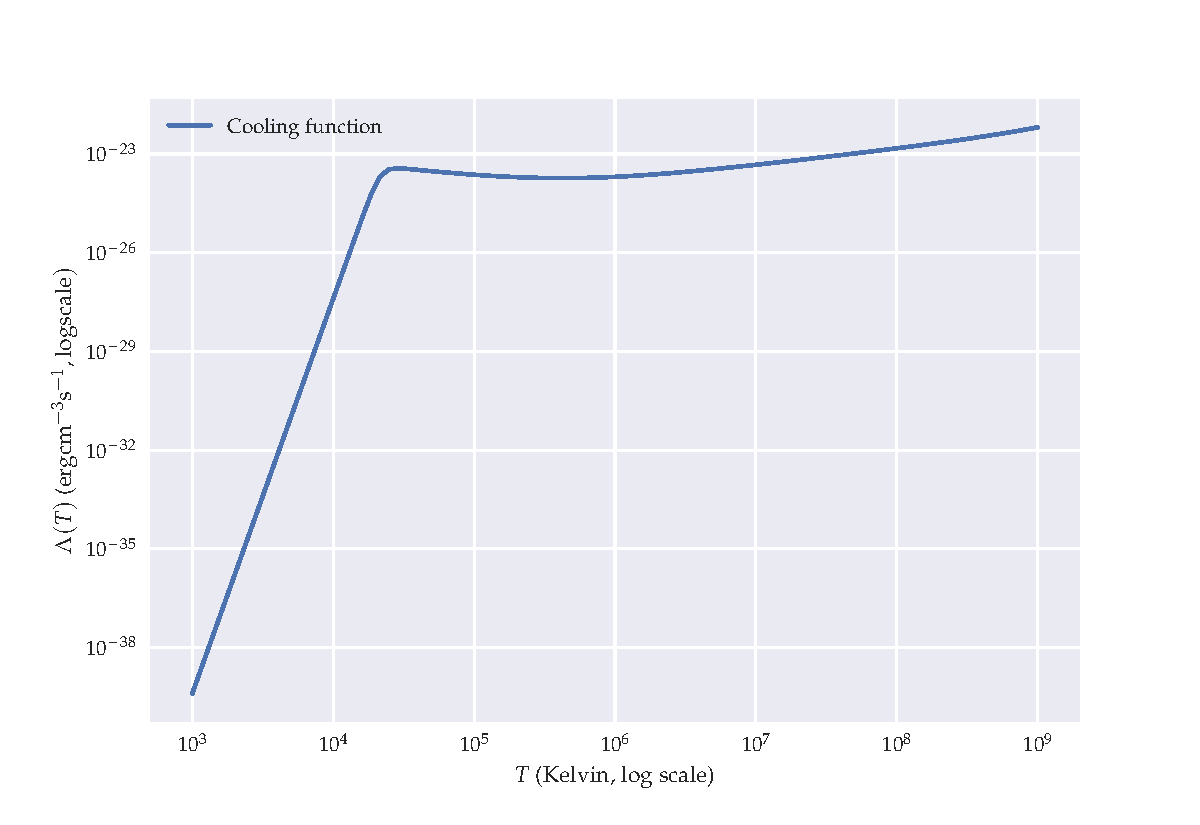
\includegraphics[width=\textwidth]{figures/cooling_function.pdf}
    \caption{Cooling function graph.}
    \label{fig:cooling-function}
\end{figure}

\begin{equation}
    \begin{split}
    \Lambda (T) &= \left(
    \qty(
    \num{1.42e-27}T^{1/2} \qty(
    1 + \num{4.4e-10}T
    ) + \num{6.0e-22}T^{-1/2}
    )^{-1} \right. \\
    & \quad \left. + \num{e25} \qty(\frac{T}{\SI{1.5849e4}{K}})^{-12}
    \right)^{-1} \si{\erg\cubic\centi\metre\per\second}
    \end{split}
\end{equation}

The version of this equation in \textcite[equation 10]{StellingwerfBuff:1982} is similar: the first constant is \(\SI{2.4e-27}{} \) instead of \(\SI{1.42e-27}{} \), and the factor \(\qty(1 + \SI{4.4e-10}{}T)\) is just \(1\).

\subsection{Thorne's PSTF moment formalism}

Following \cite{Thorne:1981feb}.

Given any tensor \(A^{\mu_1 \dots \mu_k}\) we can use the tensor \(h^{\mu\nu}\) to project it into the space-like subspace defined by the velocity \(u^\mu\):

\begin{equation}
    A^{\mu_1 \dots \mu_k} \rightarrow \qty(A^{\mu_1 \dots \mu_k})^P
    = \qty(\prod_i h^{\mu_i}_{\nu_i}) A^{\nu_1 \dots \nu_k}
\end{equation}

Then, we can take the symmetric part of any (?) tensor as outlined in \Nameref{sec:notational-preface}:

\begin{equation}
    A^{\mu_1 \dots \mu_k} \rightarrow \qty(A^{\mu_1 \dots \mu_k})^S
    = A^{(\mu_1 \dots \mu_k)}
\end{equation}

We can select the trace-free part of a projected, symmetric tensor by

\begin{equation}
    A^{\mu_1 \dots \mu_k} \rightarrow \qty(A^{\mu_1 \dots \mu_k})^{TF}
    = \sum _{i=0}   ^{\lfloor k/2 \rfloor}
    (-1)^i \frac{k! (2k-2i-1)!!}{(k-2i)! (2k-1)!! (2i)!!}
    h^{(\alpha_1 \alpha_2} \dots h^{\alpha_{2i-1} \alpha_{2i}}
    A^{\alpha_{2i+1} \dots \alpha_k) \beta_1 \dots \beta_i}\,_{\beta_1 \dots \beta_i}
\end{equation}

To see what this is doing, let us consider its action on a rank-two tensor:

\begin{equation}
    A^{\mu\nu} \rightarrow A^{\mu\nu} - \frac{1}{3} h^{\mu\nu} A^{\rho}_\rho
\end{equation}

Now, let us consider all the unit vectors \(n^\mu\) in the space normal to the velocity, which have \(n_\mu u^\mu = 0\) and \(n^\mu n_\mu = 1\). They span a three-dimensional sphere.

If we have a function \(F\colon S^2 \rightarrow \mathbb R\), we can decompose it into harmonics as such:

\begin{equation}
    F(n) = \sum _{k=0}   ^{\infty}
    \mathscr F_{\alpha_1 \dots \alpha_k} \prod_{i=0}^k n^{\alpha_i}
\end{equation}

Where the PTSF moments \(\mathscr F_{\alpha_1 \dots \alpha_k}\) can be computed as

\begin{equation}
    \mathscr F_{\alpha_1 \dots \alpha_k} =
    \frac{(2k+1)!!}{4 \pi k!} \qty(\int F \prod_{i=0}^k n^{\alpha_i}  \dd{\Omega}  )^{TF}
\end{equation}

Now, consider a photon, whose trajectory in spacetime is parametrized as \(\gamma(\xi)\), with a choice of \(\xi\) such that the photon's momentum is

\begin{equation}
    p = \dv{}{\xi}
\end{equation}

Now, our observer has a timelike velocity \(u^\mu\). We can find a spacelike vector \(n^\mu\) corresponding to the space-like part of the movement of the photon, or

\begin{equation}
    p^\mu = (- u^\nu p_\nu) (u^\mu + n^\mu)
\end{equation}

Now, we define a parameter \(l\) which corresponds to the space distance the photon moved through in this frame (this is \emph{not} covariant!)

\begin{equation}
    l = \int  (-u^\nu p_\nu) \dd{\xi}
\end{equation}

now, \(\dv*{}{l} \) is parallel to \(p\) but it has different length, in fact since \(\dv*{l}{\xi} = (-u^\nu p_\nu) \) it is \(\dv*{}{l} = u + n \).

\end{document}
